\chapter{Implementation}

The intent of this chapter is to explain and document the implementation of the CoffeeBreak system. The chapter will go over each of the eight components described in the previous Design chapter, and explain how they were implemented as well as the languages, technologies, and tools used.

All components but one are written in JavaScript using Node.js, and all use a small set of node modules to function. These modules are, in no particular order:

\begin{itemize}
    \item Express, a webserver framework used to create and provide HTTP endpoints.\cite{express}
    \item CORS\cite{expresscors}, JSON\cite{expressapi}, and cookie-parser\cite{expresscookies} middleware for the Express framework, which respectively provide CORS, JSON and cookie support.
    \item Socket.io, a high-level client-server bi-directional event based communication framework with a variety of useful features such as room and namespace support.\cite{socketio}
    \item Axios, a tool for creating and sending HTTP requests.\cite{axios}
    \item MySQL2, a framework for connecting, and making database queries, to a MySQL database.\footnote{The MySQL2 node modules was chosen over MySQL module, due to the MySQL module being outdated at the time of implementation.}\cite{mysql2}
\end{itemize}

The final non-JavaScript component is the media relay server, which is written in Python and uses a set of plugins which are outlined in the components own section of this chapter.

All chosen technologies are chosen over alternative equivalents for no particular reason other than developer preference.

The components source code are available on GitHub here: https://github.com/CoffeeBreak-Architecture/\cite{sourcecode}

\section{Main Controller - Yggdrasil}

As described in the Design chapter, Yggdrasil is responsible for providing an entryway for the rest of the system, and take in initial room requests from users. It is written in JavaScript using Node.js and Express as a web server framework, as well as a number of smaller, arbitrary modules. Being mostly boilerplate for the rest of the system, this component is simple in internal design, and the web server part consists of no more than about 80 lines of JavaScript code in total.

It needs to be linked to the room manager through the environment variable\newline$ROOM\_MANAGER\_URL$, which should point at the room manager service.

\subsection{index.js}

The entry script for the component is composed mostly of two primary Express-based HTTP endpoints, as well as an additional one needed by the Kubernetes environment for health checks. Furthermore, the Express module is requested to make use of the CORS, JSON, and cookie-parser middleware. In addition, it provides access to the socket.io node module so that clients may access the client framework.

\subsubsection{GET /room}

The first of the two primary HTTP endpoints. This is used by the client to request a new room. It functions simply by requesting the creation of a new room using the $createRoom()$ function from manager.js, and then redirecting the client to GET /room/:roomId where :roomId is the newly created rooms ID.

\subsubsection{GET /room/:roomId}

The second of the two primary HTTP endpoints. This is what clients use to connect to a particular room, such as if they have been provided a URL by a peer, or have been redirected by the previously mentioned GET /room endpoint. It works simply by requesting room from the room manager, and sending the room ID, as well as connection information, back to the client using cookies, as well as returning the room client HTML document which forms the base of the browser-based client. In this chapter, a colon prefixed in a part of the url as it is done in :roomId indicates that it the part is a parameter, and can be anything.

\begin{figure}[H]
    \centering
    \begin{subfigure}[b]{0.48\textwidth}
        \centering
        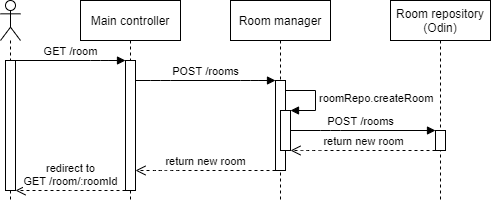
\includegraphics[width=\textwidth]{Pictures/YggdrasilNewRoom.png}
        \caption{The sequence of events when making a GET /room request for a new room.}
        \label{fig:yggdrasilgetroom}
    \end{subfigure}
    \hfill
    \begin{subfigure}[b]{0.48\textwidth}
        \centering
        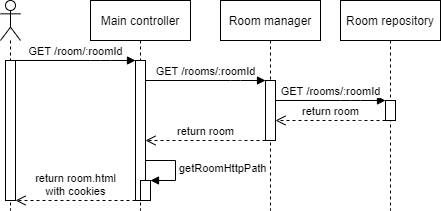
\includegraphics[width=\textwidth]{Pictures/YggdrasilGetRoom.png}
        \caption{The sequence of events when making a GET /room/:roomId request for a specific room.}
        \label{fig:yggdrasilgetspecificroom}
    \end{subfigure}
    \caption{Sequence diagram for the two major endpoints provided by the main controller. Both figures are largely similar in sequence, except for the type of request made to room manager and repositories. Notice in as well how figure a redirects to the sequence in b at the end of the sequence.}
    \label{fig:yggdrasilendpoints}
\end{figure}

\subsubsection{GET /}

This final endpoint defined by Yggdrasil is the one used by the Kubernetes environment for health checks. It merely needs to respond with anything, so as to function as a ping.

\subsection{manager.js}

The manager module is a simple Node module defined in manager.js, which provides two functions for easier and more testable access to the room manager component. The functions $createRoom()$ and $getRoom(roomId)$ are defined, and both simply use the Axios node module, a module which allows one to easily send asynchronous HTTP requests, to respectively send a POST request to the room managers POST /rooms endpoint, and a GET request to the room managers GET /rooms/:roomId endpoint.

\section{Browser-based Client - Baldr}

The browser-based client is what is used by the client to connect to and interact with the rooms themselves. It consists of a number of files provided by Yggdrasil, starting with the HTML document received when first requesting a room.

\subsection{room.html and style.css}

The room.html document is as mentioned the document first provided by Yggdrasil when requesting a room, and is where the structure of the web page itself is defined. The HTML structure is simple, and merely defines a number of <div> tags as containers to be filled out, such as list of members, a hidden list of video streams, and a chatbox for chat messages. Furthermore, it defines a large canvas which dominates the middle section of the screen, where the virtual room itself is rendered, along with the user avatars and their video streams. Finally, a chat input area is defined in the bottom of the page. The style.css document is merely a stylesheet which helps position and color the various HTML elements. An image of the resulting web page is available in figure \ref{fig:coffeebreakui} in the User Manual chapter.

\subsection{common.js}

The common.js script is a simple script with a few utility functions an an initializing $onLoad()$ function. The $onLoad()$ function listens for keydown events for the enter key, and sends the currently written chat message when the event occurs. Additionally, it sets up the canvas. Utility functions $getCookie(name)$ and $invert(object)$ are defined, which respectively provide easy access to cookies, and invert JavaScript objects.

\subsection{room.js}

The room.js script is a longer file with the primary responsibility of interacting with the room service through the socket.io client API, as well as updating all room-related information on the web page, as well as for detecting when the user clicks the room canvas. Individual units of functionality are usually only a few lines, and work to connect the end-user with the room. It connects to a remote socket.io server using a URL provided through a $socketUrl$ cookie by Yggdrasil, and listens to a number of socket events, as follows:

\subsubsection{connect}

Emitted by socket.io itself when it connects to the back-end socket server. When this occurs, the client prompts the user for a name, and emits a "login" message to the socket, along with the chosen name and ID of room the client wishes to login to. The room ID is provided to the client by the main controller as a cookie. The full sequence of events when logging in is documented in figure \ref{fig:heimdalllogin}.

\begin{figure}[H]
    \centering
    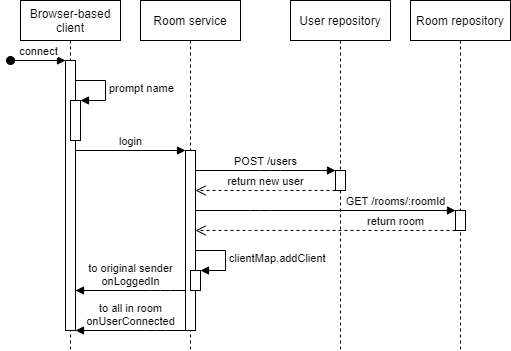
\includegraphics[width=0.65\textwidth]{Pictures/HaimdallLogin.png}
    \caption{The sequence of events when the user logs in to the room service, and how the room service makes use of an internal client map as well as room- and user repositories to register and keep track of users. Room service, client map, and the repositories are all documented later in this chapter.}
    \label{fig:heimdalllogin}
\end{figure}

\subsubsection{onLoggedIn}

Response to the $login$ message previously sent. Comes with a list of existing connected users, the ID assigned to the user, as well as room information.

\subsubsection{nearby}

Updates the client on which other users are considered "nearby", as well as the arbitrary distance threshold to be used when calculating audio gain. The client additionally calls the $callNearby()$ function which is described in the streams-p2p.js section.

\subsubsection{onUserConnected, onUserDisconnected, onMovePlayer, onChatMessage, and onNameChanged}

These all merely update the client accordingly with received information, such as adding the new user to a local list of connected users, removing users from said list, moving them, adding a chat message to the chat list, and updating a users name. Additionally triggers updates of appropriate HTML elements through a variety of utility functions.

\subsection{canvas.js}

The canvas.js script is responsible for rendering the canvas and handling clicks. The scripts functionality is implemented as a series of functions that divide-and-conquer the rendering of all the user avatars in the room, either as a simple stick figure, or as a webcam stream if one is available. Rendering is done continuously through the built-in $requestAnimationFrame(...)$ function. The sequence of function execution is documented in figure \ref{fig:rendercanvas}.

\begin{figure}[H]
    \centering
    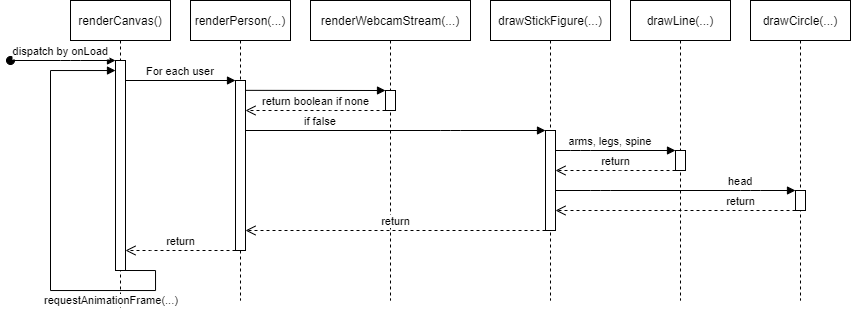
\includegraphics[width=\textwidth]{Pictures/RenderCanvas.png}
    \caption{The sequence of function execution when rendering the canvas. Shows the divide-and-conquer approach to rendering the avatars within the canvas, and how whether or not rendering video stream vs rendering a stick figure is conditional. Notice the final $requestAnitationFrame(...)$ call at the end of $renderCanvas()$.}
    \label{fig:rendercanvas}
\end{figure}

In order to handle canvas clicks, the function $onCanvasClick(...)$ subscribes to the "click" event of the canvas, which is executed when the user clicks the canvas, in order to move their avatar. This function receives information about the click event in "browser-space" as a parameter, and uses this to compute a corresponding position of the click in "world space", which the avatar is then moved to. It is worth keeping in mind that the implementation is not perfect and there is a slight offset, but it is the closest mapping after a while of trial-and-error due to unclear documentation.

\subsection{stream-players.js}
The stream-players.js script handles the media additions to the client, whether its audio or video received from the user itself or added from a remote user via WebRTC. When a media stream is received, it is split into its respective audio and video tracks. An addition to a dictionary, with the user-id as key, is created, where the respective tracks are added to for easy retrieval if required in other scripts. While the video track is only added as a video element, the audio track is used to create an $AudioContext$ and insert a $GainNode$, the latter which makes it easy to adjust the individual streams audio levels. This enables the individual user to compute the volume of each other user near them based on their distance received by the previously mentioned $nearby$ event.

\subsection{streams-p2p.js - peer to peer configuration}
The stream-p2p.js script handles the signalling and WebRTC connections between other users. When the client connects to a room it automatically connects to a socket server handling signalling. A number of events is then established client side that will execute different pieces of code depending on the message type received. In order to establish a WebRTC connection, the two users wanting to connect need to “signal” information between each other. This is done through the aforementioned signalling server. 

When the signalling starts, a Peer Connection is created. This is the object which facilitates the WebRTC connection. An offer is then sent to all users in the vicinity with the information about the created local Peer Connection, through the $callNearby()$ function. Other users receiving the offer registers the information in their Peer Connection, and sends back their information. In addition to this, the network information is also required to be shared with potential users. This is done with an event listener added to the Peer Connection. When a Peer Connection receives an ICE candidate, the client sends it automatically to all other users via the signalling server. When a clients receives an ICE candidate, it is automatically added to their Peer Connection.

In addition to handling signalling, the Stream-p2p.js script also handles dead connections. An event listener is also applied to the clients Peer Connections that checks if the connection is stopped. If it is, it is deleted and stopped. Below is a sequence diagram showcasing the WebRTC connection flow of events

\begin{figure}[ht]
    \centering
    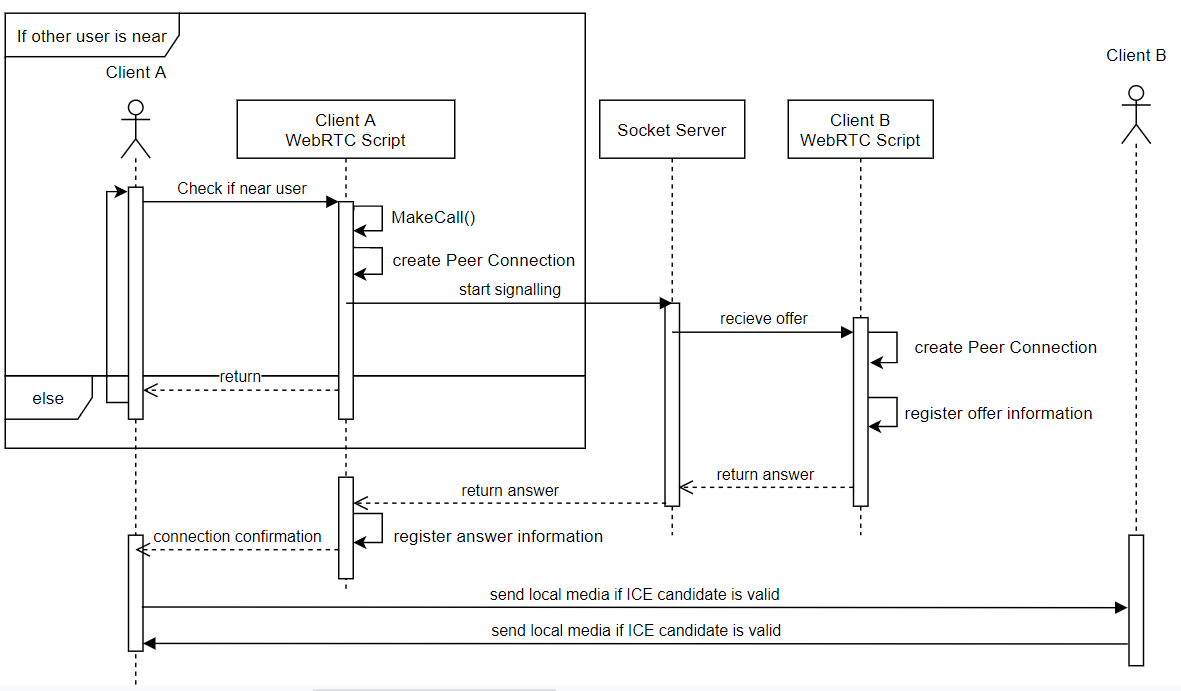
\includegraphics[width=0.85\textwidth]{Pictures/streams-p2p sequence.png}
    \caption{Sequence diagram showing the flow of events when users connect through WebRTC}
    \label{fig:gantt}
\end{figure}

\section{Room Service - Heimdall}

The room service known as Heimdall is responsible for handling the rooms themselves and the users connected to them. It is as most other services written in JavaScript using Node.js. The service is split in two major modules, rooms.js for handling rooms themselves, and signalling.js for signalling between users. Both these modules use socket.io, and socket.io namespaces to differentiate from one another. Additionally, a clientMap.js module is used to provide persistent mapping between client IDs and the IDs used internally by socket.io. Two repository modules provide access to user and room repository services. The index.js entry script is merely responsible for initializing the rooms and signalling modules with socket.io.

It needs a number of environment variables to function. A set of variables for connecting to a database: $MYSQL\_HOST$, $MYSQL\_USER$, $MYSQL\_PASSWORD$, and $MYSQL\_DATABASE$ to be set up according to MySQL specifications. Additionally, it needs the environment variables $USER\_REPOSITORY$ and $ROOM\_REPOSITORY$ to be URLs of respectively user- and room repository services.

\subsection{rooms.js}

This module is the most complex of Heimdall and as mentioned is responsible for the rooms themselves, and the users connected to them. It can be considered the server-side equivalent of the room.js script from the browser-based client, and handles all of the room-specific events. It consists primarily of following five event listeners listening to emissions from clients.

\subsubsection{login}

Emitted by the client when they wish to login to a particular room. It proceeds to request the creation of a new user from the user repository, as well as fetch room information and room members. The client is added to the clientMap modules client map. Room information, members, user information is all emitted to the client through the "onLoggedIn" event. Additionally, the "onUserConnected" event is emitted to the entire room in question, with information about the new user. The full sequence is available in figure \ref{fig:heimdalllogin}

\subsubsection{onChatMessage}

Emitted by clients when sending a chat message. Merely relays chat message to the rest of the clients in the sending clients room.

\subsubsection{onMovePlayer}

Emitted by the client when moving their avatar. Updates the clients user information through the user repository, and fetches an array of the users considered "nearby" to the client. Relays the movement to the rest of the clients room, and finally emits the "nearby" event to the client, with the array of nearby users.

\subsubsection{onNameChanged}

Emitted by the client when requesting to change their name.\footnote{This feature is left out of the final version of the browser-based client, but the functionality is left in behind-the-scenes in case it would be re-implemented in the client.} Merely updates the clients users name through the user repository, and relays the new name to all other clients in the clients room.

\subsubsection{disconnect}

Emitted by socket.io itself when a client socket is disconnected. Requests the deletion of the user from the user repository, and relays the disconnection to all other clients in the clients room through the "onUserDisconnected" event.

\subsection{signalling.js}

This module is responsible for providing signalling between users, or users and the media relay server, so that they may call each other in order to open WebRTC connections. The module listens to two events emitted by clients, "login" and "message". "login" is emitted by the clients when logging in to to the room similarity to the rooms module, though it merely adds the client to the client map. The "message" event on the other hand receives a message which has information about a sender, the ID of an intended receiver, a type, and a payload. Though the client map, the module finds out which connected socket to send the message to, and sends it.

\subsection{clientMap.js}

This module provides a set of functions for storing and accessing mappings between client IDs and the IDs used internally by socket.io to differentiate clients. The mappings are stored in MySQL database, with each mapping consisting of a socket ID, a client ID, and which namespace the mapping belongs to. The database is directly accessed using the MySQL2 module. This is used extensively throughout the service.

\subsection{userRepo.js and roomRepo.js}

These two modules are merely responsible for providing access to the user- and room repository services. They use Axios to make the HTTP requests.

\section{Room Manager Odin}

The "Odin" room manager is responsible for creating simple client-server type rooms with P2P voice/video communication. The service very simple, consisting of barely 40 lines of JavaScript split into the index.js entry script, and the roomRepo module. It uses the Node.js framework, as well as Express to provide two webserver endpoints. These two endpoints are "POST /rooms" and "GET /rooms/:roomId", the first of which requests the creation of a new room through the roomRepo module, while the other requests a particular room through the roomRepo module, and either returns the room, or a status code 404 if the requested room could not be found. The roomRepo module uses Axios to make HTTP requests, and the rooms created contains connection information which is predefined through environment variables, with this connection information usually pointing at the Heimdall room service.

This component merely needs two environment variables. $ROOM\_REPOSITORY\_URL$ pointing at the room repository service, and $SOCKET\_SERVER\_URL$ pointing at the room service, to provide as connection information to the clients.

\section{Room Repository - Huginn}

The room repository is a simple service designed to be RESTful access to CRUD room resources. It provides a layer between the rest of the system and the databases in which persistent data is stored. As with most other services, it is written in JavaScript using Node.js, and Express for providing endpoints. It uses the MySQL2 node module to connect to a MySQL database. The database is automatically initialized on first connection, if it is not already initialized, thus avoiding cumbersome database setup during deployment and testing.

This component needs environment variables to know how to connect to its database. The variables $MYSQL\_HOST$, $MYSQL\_USER$, $MYSQL\_PASSWORD$, and\newline$MYSQL\_DATABASE$ needs to be filled out according to MySQL specifications.

\section{User Repository - Muninn}

The user repository is almost identical in implementation to the room repository Huginn, except naturally that it provides CRUD access to user resources instead.

\section{Media Relay Server - Sleipnir}

The Sleipnir service is a MRS implementation, created using the AioRTC python library. Instead of users connecting to each other directly, they connect to this MRS. When a user joins a room they automatically connect to the MRS as a client. This is the users local media being sent to the server for other users to connect to. This media is then played using a MediaBlackhole which takes in media streams, plays them, and then discards the tracks. The clients media tracks are saved to the server in a client dictionary that takes the clients userid as key. These tracks are added to a MediaRelay, of which can be subscribed to, granting easy access to the clients media tracks to multiple users. When a client is nearby another client, a listener connection is established for each client. A listener connection receives the corresponding media tracks in the client dictionary and subscribes to the MediaRelay. These tracks are then added to the listener Peer Connection as their local tracks and then triggers the client remote stream event listener. Below is two sequence diagrams illustrating the functionality

\begin{figure}[ht]
    \centering
    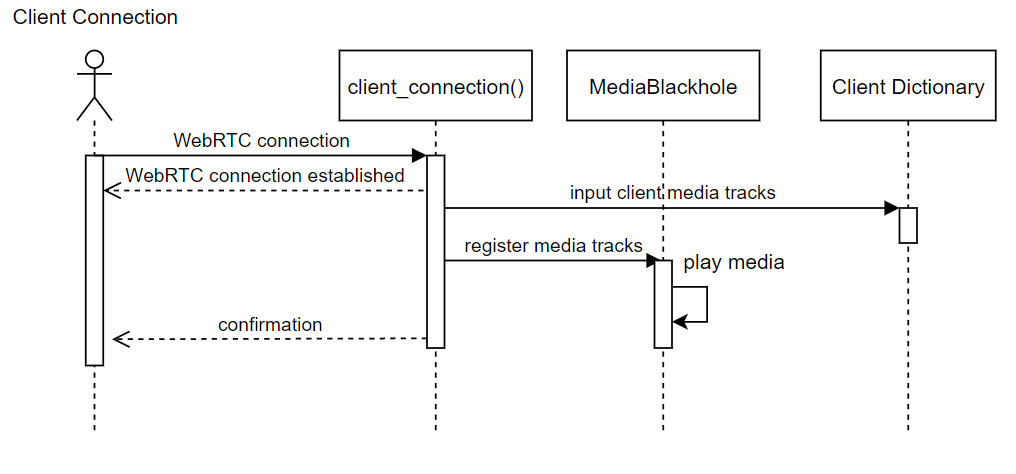
\includegraphics[width=0.8\textwidth]{Pictures/Client connection.png}
    \caption{Sequence diagram showing the flow of events when connecting as a client}
    \label{fig:gantt}
\end{figure}

\begin{figure}[ht]
    \centering
    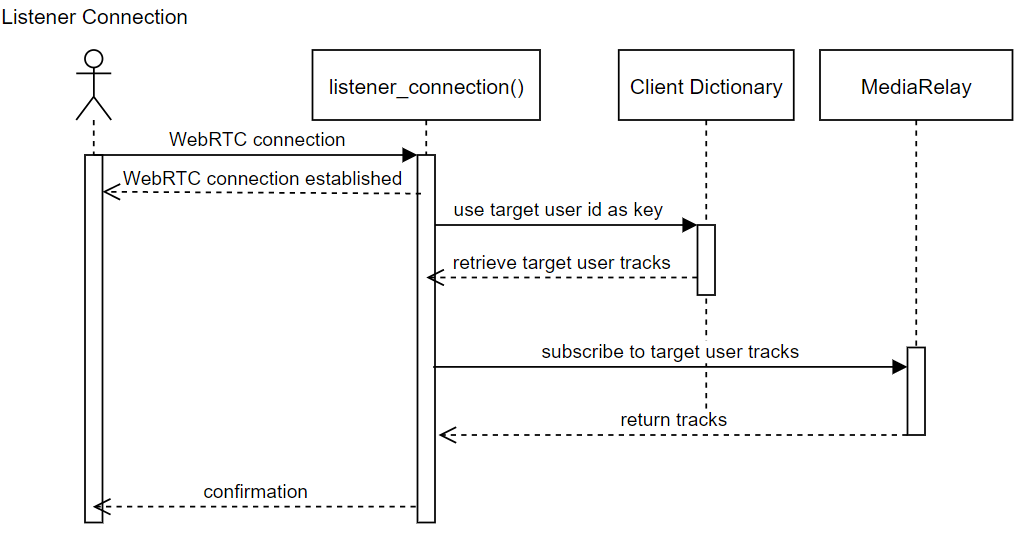
\includegraphics[width=0.8\textwidth]{Pictures/listener connection.png}
    \caption{Sequence diagram showing the flow of events when connecting as a listener}
    \label{fig:gantt}
\end{figure}

\newpage
\subsection{Client Side changes - MRS configuration}

The main functionality of the WebRTC connection is the same. However signalling is not done using the signalling server, but a series of CRUD operations between the MRS and the Client. When the user connects to a room a client connection is established, and Peer Connection information is sent between the MRS and the client The Client then awaits ICE candidates until all candidates is gathered and then returns the information to the MRS. 

If a client, A, moves near another client, B,  a listener connection is established. A connection is requested with Client B's media tracks, while a signal is sent using the socket server to Client B, which then establishes a connection with Client A's media tracks. This is illustrated with the sequence diagram below.
\begin{figure}[H]
    \centering
    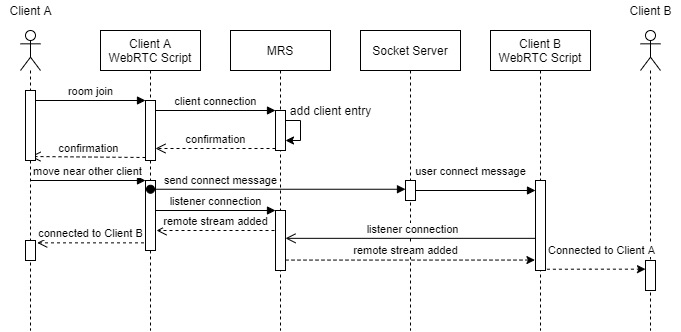
\includegraphics[width=0.8\textwidth]{Pictures/Sleipnir Configuration.png}
    \caption{Sequence diagram showing the sequence of events when connecting to the MRS in the Vili design}
    \label{fig:gantt}
\end{figure}